\newpage
\subsection{Multivariate Analysis}

\quad The Multivariate Analysis is similiar to the Univariate Analysis, the diference is that in this one we will use more than a set of data, in this project we will use the precipitation and the maximum temparature to assiste in the prediction of sales for each of the drinks.\\


For the Multivariate Analysis we create a neural network to assist in the prediction of sales for each of the drinks:

\begin{figure}[H]
    \centering
    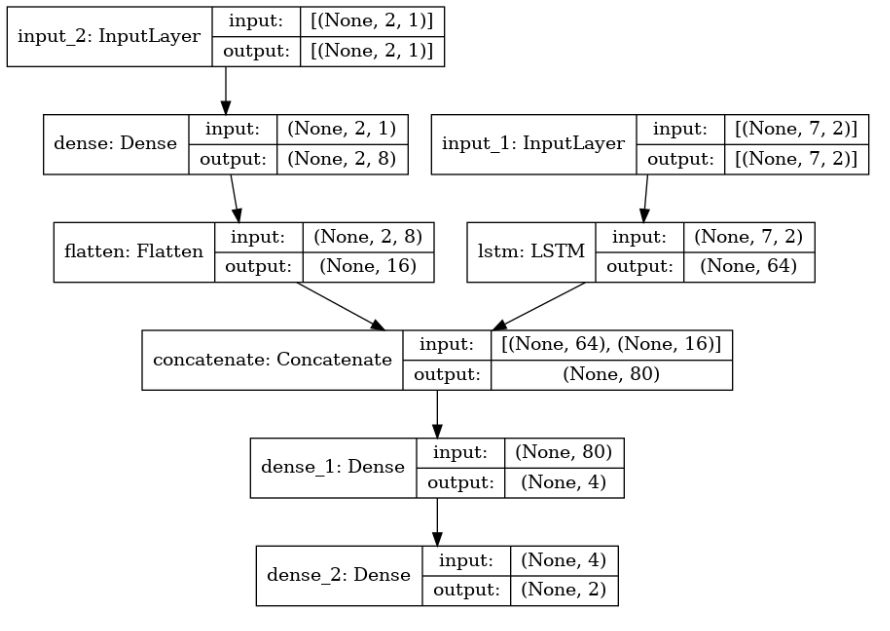
\includegraphics[width=0.8\textwidth]{assets/rede neuronal.jpeg}
    \caption{Neural Network}
    \label{fig:neural_network}
    \end{figure}


For the prediction we will use a split of Growing Window to predict the last 20 weeks of sales, for each drink, with a step of 7. The next image represents the results of the error mean of the 20 weeks prediction:\\


\begin{figure}[H]
    \centering
    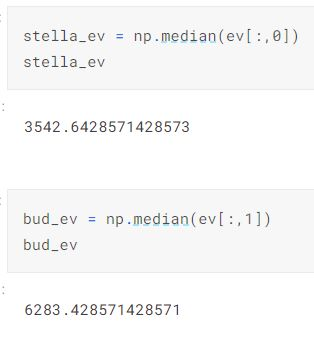
\includegraphics[width=0.4\textwidth]{assets/erros-previsao.jpeg}
    \caption{Mean of MSE Error for STELLA and BUD}
    \label{fig:notas}
    \end{figure}

For demonstration purposes here are the graphics of each of the predictions made for the BUD and STELLA:\\

\begin{figure}[H]
    \centering
    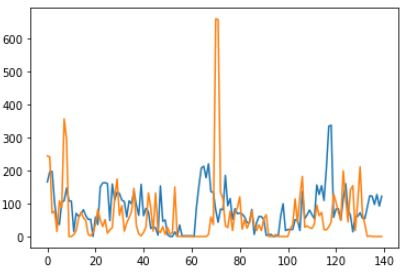
\includegraphics[width=0.6\textwidth]{assets/multi-stella.jpeg}
    \caption{STELLA - Multivariate Analysis Results}
    \label{fig:notas}
    \end{figure}

\begin{figure}[H]
    \centering
    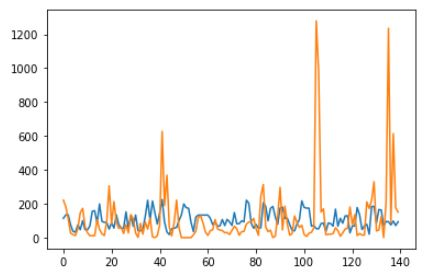
\includegraphics[width=0.6\textwidth]{assets/multi-bud.jpeg}
    \caption{STELLA - Multivariate Analysis Results}
    \label{fig:notas}
    \end{figure}







